
\subsection{Simulation Results}

Corollaries \ref{cor: consequence of main theorem 1}, \ref{cor: consequence of main theorem 2}, and \ref{cor: consequence of main theorem 3} provide theoretical guidance on the optimal choice of $\lamz$ to minimize the upper bound on excess risk. However, while these results bound the theoretical risk, they do not guarantee that the same value of $\lamz$ is optimal for the true excess risk in practice. To investigate this, we conduct empirical simulations to identify the values of $\lamz$ that minimize the actual excess risk.

Our simulation study evaluates the empirical behavior of the optimal regularization parameter, $\lamz$, across two distinct scenarios: a synthetic toy dataset and a collection of real-world datasets.

\subsection{Toy DataSet}
We generate $100$ different distributions over $(X, Y, Z)$, each constructed as follows:

\begin{enumerate}
    \item The features $X$ are sampled from a Gaussain mixture model, whose parameters and mixing probabilities are randomly choosen.
    
    \item Then the weight vectors $u$ and $w$ are sampled from standard normal distribution.    
    Given fixed weights $u$, the binary variables $Z$ is sampled via logistic models:
    \[ Z \sim \sigma((1,X)^\top u).\]
    Once we get $Z$, then for a fixed weight $w$, the binary variable $Y$ is sample via logistic model:
    \[ Y \sim \sigma((1,X,Z)^\top w).\]
    
\end{enumerate}

This process is repeated $100$ times, each with a new random choice of parameters, resulting in a diverse family of distributions for evaluating the bang-bang behavior of the optimal $\lamz$.

For each distribution, we generate $m=1000$ samples for the $(X, Z)$ dataset (used for learning $X \to Z$), $n=4000$ samples for the $(X, Y)$ dataset (used for learning $X \times Z \to Y$), and $t=20000$ samples for the test set $(X, Y, Z)$ to compute the excess risk. 
For each value of $\lamz$ in the candidate set
\begin{equation*}
    \{0.01, 0.1, 1.0, 10.0, 100.0, 1000.0, 10000.0, 100000.0\},
\end{equation*}
a model is trained and evaluated. The optimal $\lamz$ for each distribtution is chosen as the value that yields the lowest empirical excess risk on the test set.

The frequency of each candidate $\lambda$ value being chosen as the optimal $\lamz$ across the $100$ distributions is shown in Figure \ref{fig: lambda plot}. The simulation results, summarized in the frequency plot, show a strong preference for the extreme values of the regularization parameter $\lamz$. This observed bang-bang behavior of $\lambda_z$ provides empirical evidence suggesting a bang-bang nature of $\lambda_z$.

\begin{figure}[htbp]
\centering
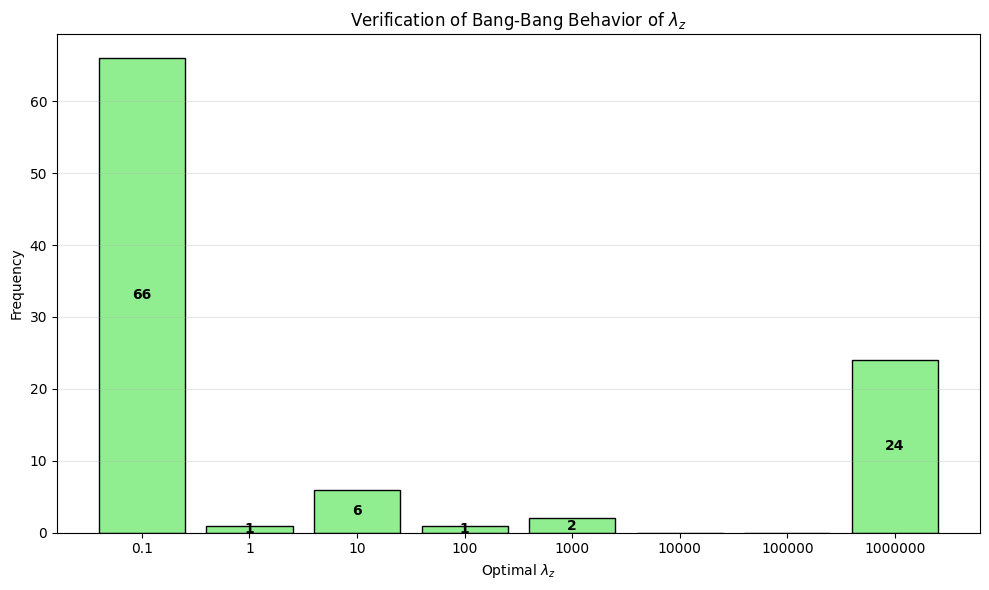
\includegraphics[scale=0.5]{lambda_frequency.png}

\caption{Frequency of optimal $\lamz$ values across 100 independent simulation seeds. For each seed, $\lamz$ is the value from the set $\{0.1, 1, 10, 100, 1000, 10000, 100000, 1000000\}$ that minimizes the empirical excess risk.}
\label{fig: lambda plot}

\end{figure}
\FloatBarrier




\subsection{Real World Data Set}

To validate the bang-bang behavior in practical settings, we evaluate the optimal regularization parameter $\lamz$ across nine real-world datasets from the OpenML repository. For each dataset, we identify a primary target variable $Y$ and a relevant binary side attribute $Z$, as described below:

\begin{enumerate}[label=(\roman*)]
    \item \textbf{Adult Income ($n=48,842$):} $Y$ is Income, $Z$ is Sex, and $X$ comprises demographic and employment attributes.
    \item \textbf{Bank Marketing ($n=45,211$):} $Y$ is Term Deposit subscription, $Z$ is Housing Loan status, and $X$ contains client and contact data.
    \item \textbf{German Credit ($n=1,000$):} $Y$ is Credit Risk, $Z$ is Foreign Worker status, and $X$ captures personal financial attributes.
    \item \textbf{Titanic Survivor ($n=1,045$):} $Y$ is Survival, $Z$ is Sex, and $X$ includes passenger class, age, and fare.
    \item \textbf{Breast Cancer ($n=699$):} $Y$ is Malignancy, $Z$ is Clump Thickness, and $X$ consists of cell nuclei measurements.
    \item \textbf{Diabetes ($n=768$):} $Y$ is Diabetes positive status, $Z$ is Age, and $X$ involves medical metrics.
    \item \textbf{Spambase ($n=4,601$):} $Y$ is Spam classification, $Z$ is word frequency of "make", and $X$ includes various word and character frequencies.
    \item \textbf{Sick ($n=3,772$):} $Y$ is Thyroid diagnosis, $Z$ is Sex, and $X$ covers thyroid clinical measurements.
    \item \textbf{Mushroom ($n=8,124$):} $Y$ is Edibility, $Z$ is Bruises, and $X$ records morphological traits.
\end{enumerate}

We employ a 70/30 train-test split for each dataset. The training portion is further partitioned using a 79:21 ratio to form the primary dataset $D$ ($n$ samples) and the side information dataset $S$ ($m$ samples). We utilize Logistic Regression models (L-BFGS) for both imputation mapping ($X \to Z$) and primary classification. The optimal $\lamz$ is determined by evaluating the excess risk on the test population over a logarithmic grid ranging from $10^{-3}$ to $10^{5}$.

The results, summarized in Figure \ref{fig: real world plot}, confirm that for all nine datasets, the optimal regularization parameter $\lamz$ concentrates at the extreme boundaries of the search grid, providing strong empirical evidence for the bang-bang nature of $\lambda_z^*$ in diverse real-world distributions.

\begin{figure}[htbp]
\centering
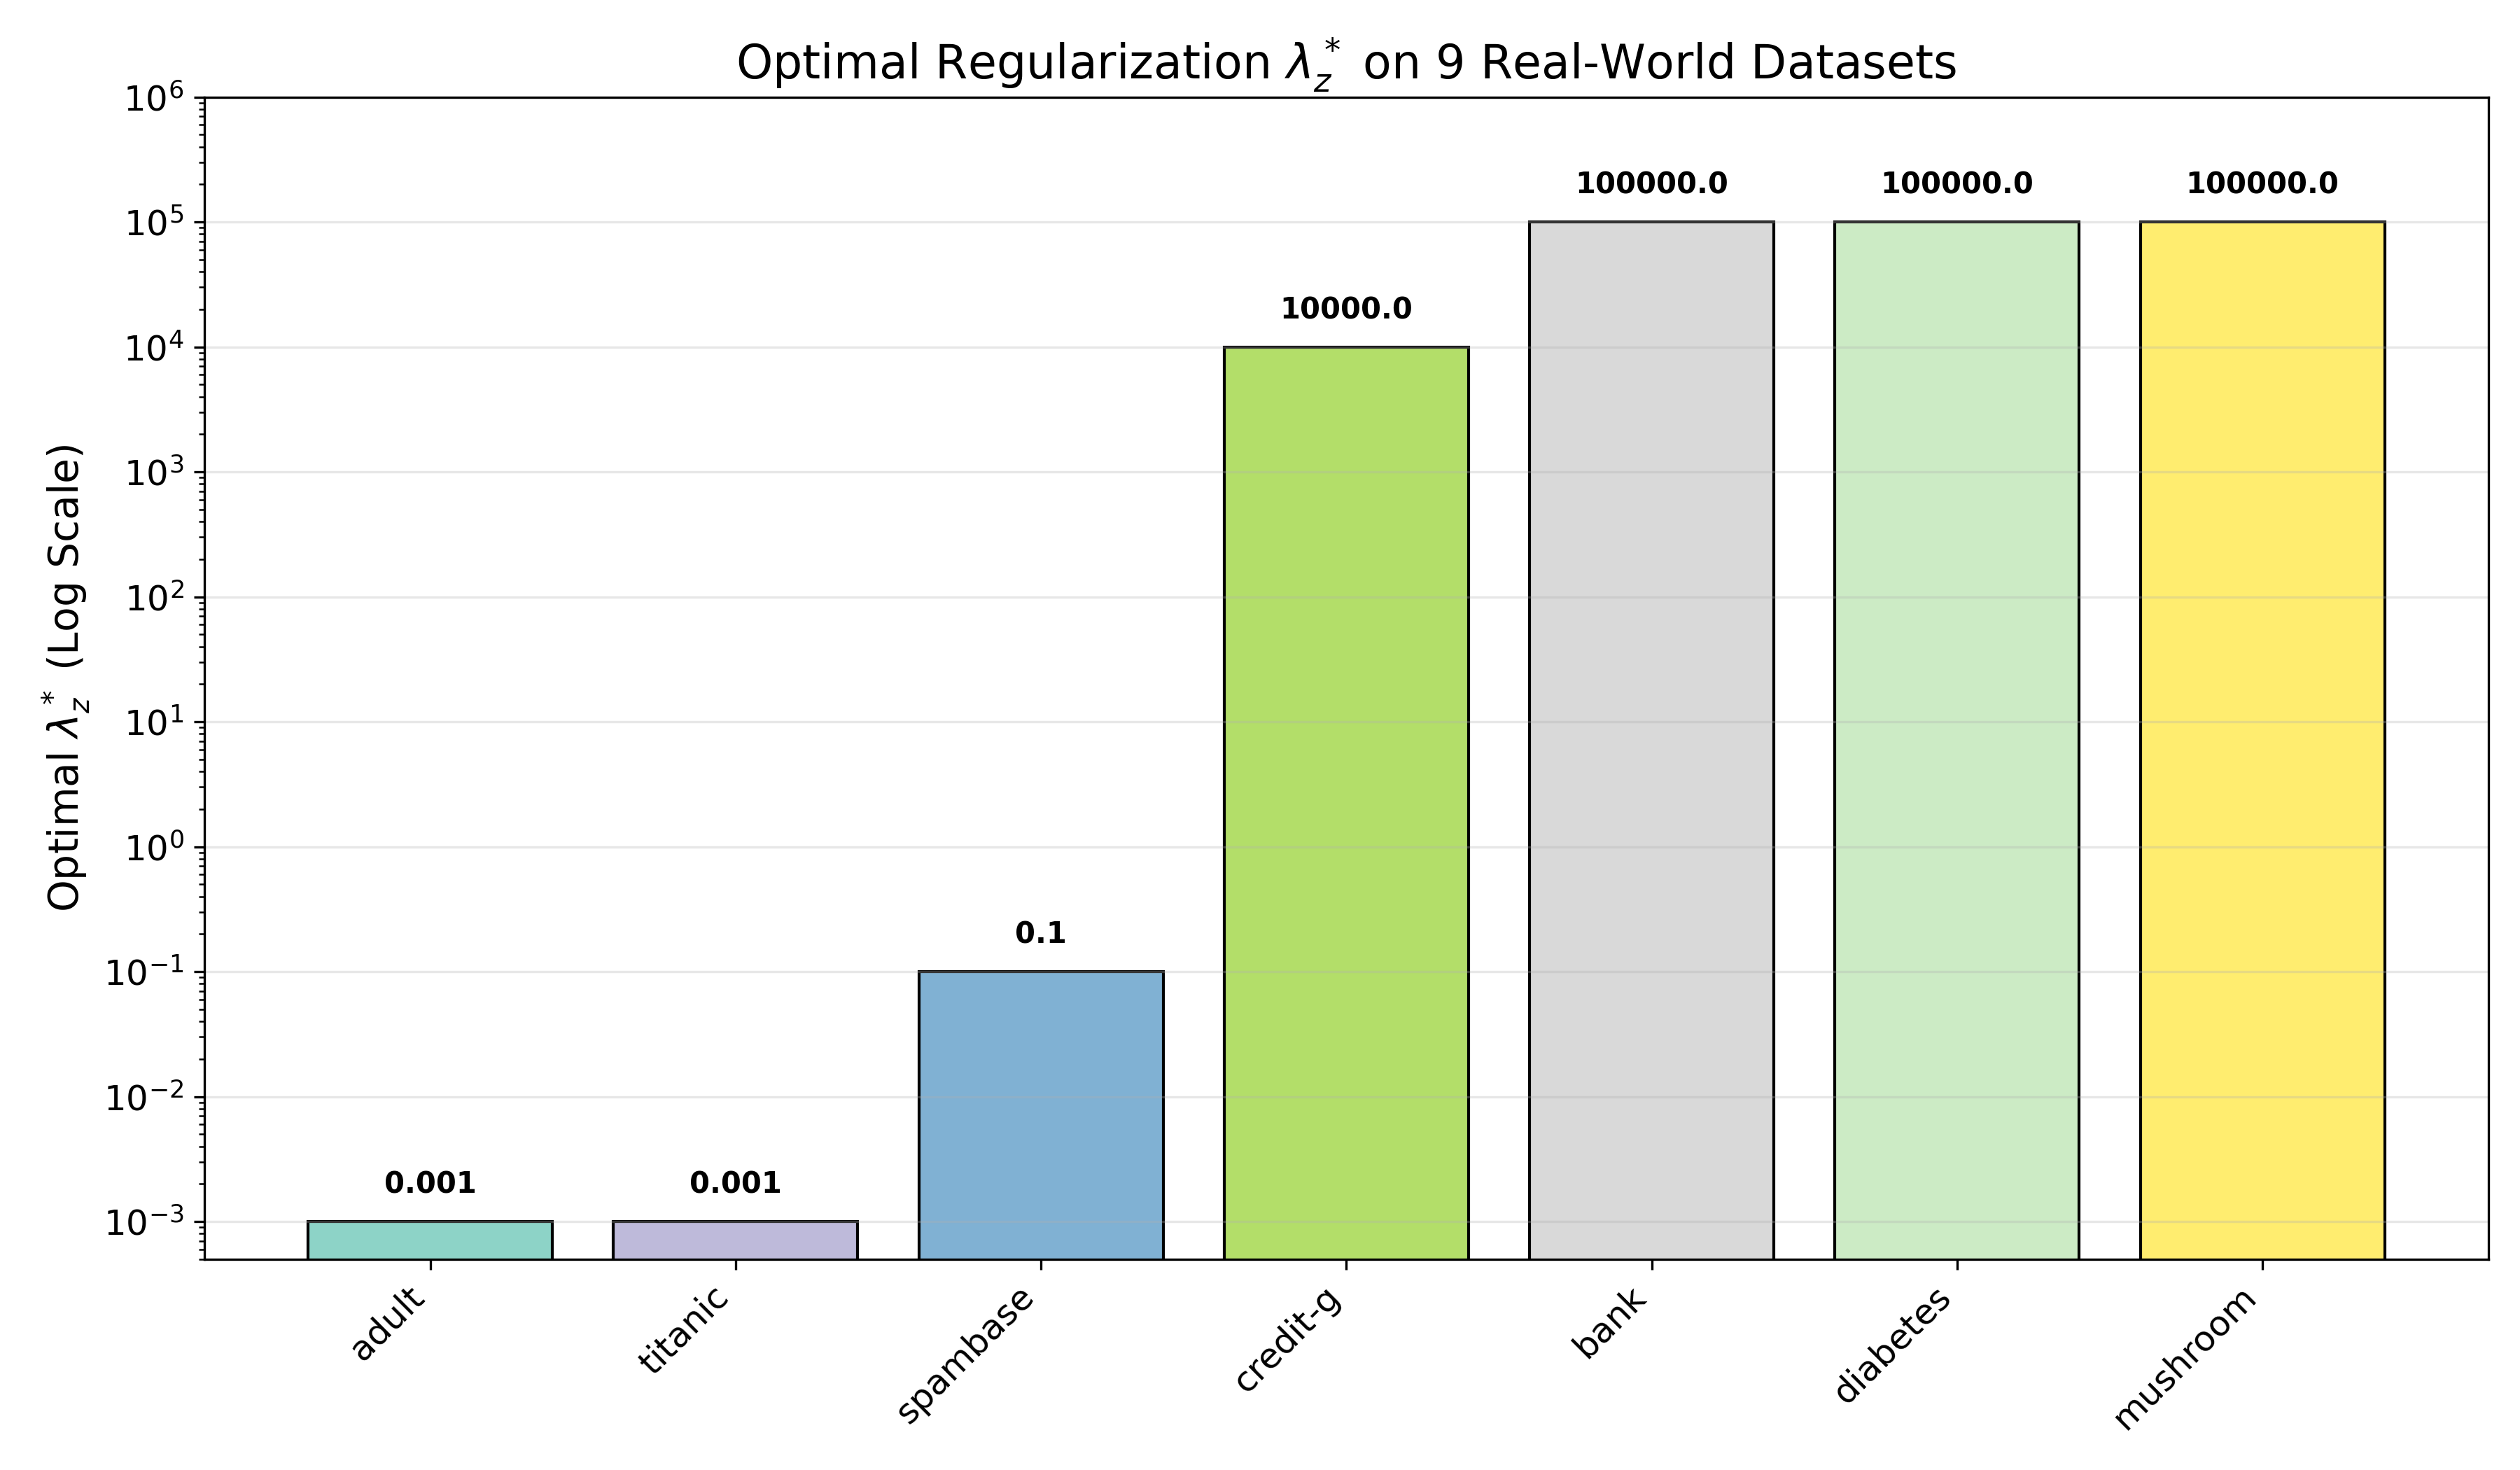
\includegraphics[scale=0.5]{Real_World_Experiments/optimal_lambda_real_world.png}
\caption{Optimal regularization parameter $\lambda_z^*$ across 9 real-world datasets. The values are sorted in ascending order of the optimal $\lambda_z$. In all cases, the optimum is found at the boundaries of the candidate grid.}
\label{fig: real world plot}
\end{figure}
\FloatBarrier